\documentclass[11pt,a4paper]{article}
\usepackage[margin=2.2cm]{geometry}
\usepackage[T1]{fontenc}\usepackage{lmodern}
\usepackage{amsmath,amssymb,booktabs,tabularx,longtable,float}
\usepackage{tikz,pgfplots}\usetikzlibrary{positioning}\pgfplotsset{compat=1.18}
\usepackage{xcolor}\definecolor{accent}{HTML}{164B68}
\usepackage{hyperref}\hypersetup{colorlinks=true,linkcolor=accent,urlcolor=accent}
\usepackage{fancyhdr}\pagestyle{fancy}\fancyhf{}\fancyhead[L]{KuaiRand-Pure | Week 1}\fancyhead[R]{Measured baseline -- report revision}\fancyfoot[C]{\thepage}\setlength{\headheight}{14pt}
\setlength{\parskip}{.5em}\setlength{\parindent}{0pt}
\setlength{\emergencystretch}{2em}
\begin{document}
\begin{titlepage}
\centering\vspace*{1.3cm}
{\Huge\bfseries KuaiRand-Pure\\[.3cm]Week 1 Technical Report\par}
\vspace{.5cm}{\Large Two-Tower Retrieval Baselines and Evaluation\par}
\vspace{.5cm}{\large SAR Recommendation Project\par}
\vspace{.7cm}\fbox{\strut Measured baseline -- report revision}
\vspace{1cm}
\begin{minipage}{.88\textwidth}
\textbf{Abstract.} This work implements a reproducible long-view retrieval baseline on the official Pure candidate pool. The system checks source identities, removes exact raw duplicates, rebuilds histories using observed playback completion, trains normalized user/item towers, exports aligned vectors and evaluates deterministic exact Top-100 retrieval. The corrected comparison evaluates 30,589 held-out requests: popularity achieves Recall@100 0.270784, basic 0.020301 and enhanced 0.019288. Both neural runs complete the same one-epoch budget, and controlled CUDA checkpoint recovery matches the uninterrupted enhanced state exactly. Standard-exposure offline metrics describe held-out logged positives; they do not establish an online business improvement.

\medskip\textbf{Current evidence.} The corrected dataset contains 124,255 training positives and 30,589 validation-positive requests, against 7,583 candidate items. All three baselines are measured on this protocol in the completed Colab release. The earlier published enhanced checkpoint is retained as a separate historical diagnostic because its duplicate and history rules differ.

\medskip\textbf{Acceptance status.} The experiment stage reports complete with no artifact blockers. This certifies the recorded runs and controlled recovery check; it does not establish model superiority, online benefit or recovery after rebuilding a Colab runtime. This report revision incorporates the completed evaluation evidence.
\end{minipage}
\vfill{\large Generated from versioned experiment artifacts\par}
\end{titlepage}
\section{Problem framing and supervision}
At request time $t$, the system receives an anonymous user identifier, a scenario identifier and previously available positive feedback. It returns up to 100 videos from a time-eligible catalog. This is a \textbf{candidate-retrieval problem}: a user encoder and an item encoder map inputs into a common 64-dimensional space.

\subsection{Target and unit of evaluation}
The target is official $\texttt{long\_view}=1$ in standard, nonrandom exposure. For videos no longer than 18 seconds, the label requires watching at least the video's duration; for longer videos it requires at least 18 seconds. The label is copied from the official logs, not regenerated from our feature snapshot. One positive logged exposure is one evaluation request with one relevant item.

The learned score is normalized dot product,
\[s(u,i)=\langle f_\theta(u,t,h),g_\phi(i)\rangle,\qquad \|f_\theta\|_2=\|g_\phi\|_2=1.\]
It is a ranking score, not a calibrated probability of long viewing. The model learns to rank a positive target above eligible comparison examples, rather than fitting an explicit positive/negative binary classifier on all exposures.

\subsection{Why the baseline has three components}
Popularity measures how far training-period positive frequency alone can go. The basic neural model uses user ID and request context with an ID-only item tower. The enhanced model adds a masked mean of positive history. Both neural runs share data, shuffle seed, output dimension and optimizer budget. Unversioned item content is excluded from the corrected comparison; the earlier content model is documented separately.

\subsection{Interpretation boundary}
Pure contains only logs involving the published candidate pool, so its histories omit other watched videos. Main validation uses standard exposure and can inherit its selection bias. Random exposure is kept separate, and the final test bundle remains sealed. The work does not claim unbiased online retention, CTR or revenue improvement.
\clearpage
\section{Dataset and exploratory analysis}
The source is the official KuaiRand-Pure archive. Its official MD5 is checked before processing. The shared Drive event/history/feature files are additionally matched to their frozen SHA-256 values. Raw event identities and primary fields are compared to the published event table before any new training artifacts are written.

\begin{table}[H]\centering\small
\begin{tabular}{lrrrrr}\toprule
Window & Exposures & Positives & Positive rate & Users & Items\\\midrule
warmup & 886,326 & 297,920 & 33.61\% & 25,185 & 7,521 \\
train & 363,643 & 124,255 & 34.17\% & 25,769 & 6,882 \\
validation & 94,578 & 30,589 & 32.34\% & 20,565 & 5,279 \\
\bottomrule\end{tabular}\caption{Retained nonrandom warmup/train/validation data after exact full-row deduplication. Counts are unique within each window; users/items can overlap across windows.}\end{table}

Training-period item positive counts have median 6, 95th percentile 101 and maximum 1,135. The top 100 items account for 26.83\% of training positives. This concentration motivates the popularity comparator.

Training-user exposure counts have median 10 and 95th percentile 40. These are exposure counts, not the number of optimizer updates per user.

Observed video-duration quantiles (seconds) are: median 70.60, 75th percentile 139.43, and 95th percentile 288.60. The raw duration includes zero values; these are retained and reported, not replaced by a guessed duration.
\begin{figure}[H]\centering
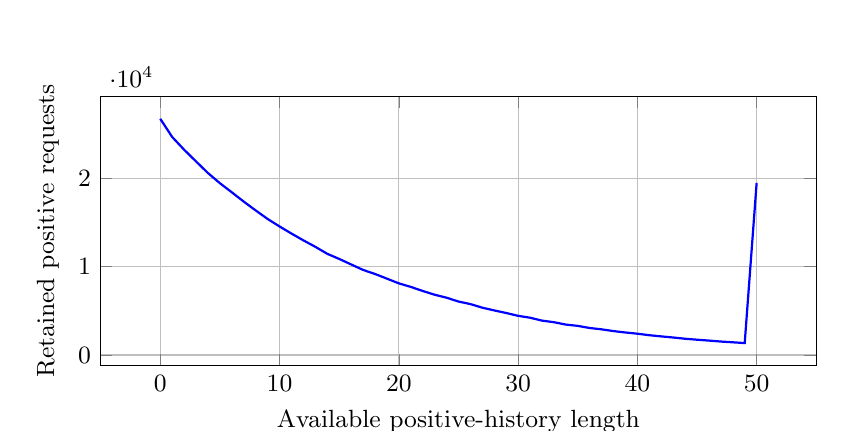
\begin{tikzpicture}\begin{axis}[width=.88\linewidth,height=5cm,
  xlabel={Available positive-history length},ylabel={Retained positive requests},grid=major,
  tick label style={font=\small},label style={font=\small}]
\addplot[color=blue,thick] coordinates {(0,26722) (1,24662) (2,23220) (3,21896) (4,20582) (5,19434) (6,18402) (7,17350) (8,16354) (9,15389) (10,14541) (11,13737) (12,12969) (13,12240) (14,11449) (15,10870) (16,10247) (17,9626) (18,9169) (19,8641) (20,8105) (21,7707) (22,7244) (23,6821) (24,6484) (25,6051) (26,5762) (27,5355) (28,5045) (29,4753) (30,4433) (31,4220) (32,3892) (33,3714) (34,3442) (35,3298) (36,3055) (37,2905) (38,2706) (39,2549) (40,2411) (41,2241) (42,2106) (43,1982) (44,1840) (45,1732) (46,1632) (47,1525) (48,1439) (49,1352) (50,19463)};
\end{axis}\end{tikzpicture}\caption{History-length distribution across retained warmup/train/validation positives; maximum length 50. Zero-history rate is 5.90\%.}\end{figure}
\clearpage
\section{Preprocessing and temporal audit}
\subsection{Existing preparation}
The publisher maps original anonymous IDs, timestamps, scenario, official label and random flag into standardized events. It assigns time splits and prepares static item metadata plus request-prior positive histories. The earlier consumer fits categorical dictionaries and numeric transformations from training-referenced items rather than the entire catalog.

\subsection{Corrections introduced for this stage}
The new audit removes 20,624 rows that are equal across \emph{all} raw CSV columns, while retaining other repeated watches. Request IDs preserve the original filename and row number. No heuristic user-item deduplication is applied.

Histories now require
\[t_{\mathrm{available}}=t_{\mathrm{request}}+\texttt{play\_time\_ms}
<t_{\mathrm{current\ request}}.\]
The inequality is strict: a completion at the same millisecond is unavailable. A delayed completion is inserted in original request order, and the last 50 available positive observations are retained. The completion rule changes 1,038 histories relative to request-prior histories on the same deduplicated events. Random observations never become main-training histories.

This is a \textbf{conservative observed-playback proxy}. The source does not provide an independent feedback ingestion timestamp; therefore the audit does not claim exact production feedback availability.

\subsection{Calendar consistency}
Recorded date differs from timestamp-derived dates on 196,989 retained exposures under UTC and 11,235 under UTC+08. We do not silently declare either source calendar verified. Splits and periodic context instead use the explicit UTC timestamp protocol below.

\begin{center}\begin{tabular}{ll}\toprule
Warmup & $t < $ 2022-04-15 00:00 UTC\\
Train & 2022-04-15 00:00 $\le t <$ 2022-04-29 00:00 UTC\\
Validation & 2022-04-29 00:00 $\le t <$ 2022-05-04 00:00 UTC\\
Test & Sealed; excluded from fitting and this report's EDA\\\bottomrule
\end{tabular}\end{center}
\clearpage
\section{User-side features and actual encodings}
\begin{table}[H]\centering\small
\begin{tabularx}{\linewidth}{lXll}\toprule
Feature & Source/meaning & Raw type & Encoded width\\\midrule
User ID & Anonymous training-window ID dictionary & int64 & 32\\
Scenario/tab & Request scenario; valid range 0--14 & int64 & 8\\
Request time & Unix milliseconds; day/week cyclic context & int64 & 4\\
Positive history & At most 50 available prior item IDs & list[int64] & 64 pooled\\
History mask & Valid history slots; padding is excluded & bool[50] & mask only\\\bottomrule
\end{tabularx}\caption{User inputs. Basic omits history; enhanced includes its 64-dimensional masked mean.}\end{table}

User dictionaries are fitted to training-window users only and are numerically sorted. Known IDs map to indices $1,\ldots,V_u$; unseen users use index 0. This reserved embedding has no guaranteed learned cold-start behavior, so unknown-user coverage is reported explicitly. Tab values map to $\texttt{tab}+1$; out-of-range scenarios use reserved index 0.

For timestamp $T$ in milliseconds, with a zero UTC offset,
\begin{align*}
\alpha_d &=2\pi\,(T/1000\bmod86400)/86400,\\
\alpha_w &=2\pi\,((T/1000+3\cdot86400)\bmod604800)/604800.
\end{align*}
The four values are $(\sin\alpha_d,\cos\alpha_d,\sin\alpha_w,\cos\alpha_w)$. The three-day shift aligns the Unix epoch's Thursday with a Monday-based week. An actual retained timestamp, \texttt{1649475963278}, produces approximately
\[0.834017,\quad 0.551738,\quad -0.996517,\quad -0.083395.\]

Historical raw item IDs are left-padded with $-1$, distinct from real raw item ID 0. The shared item encoder generates $[B,50,64]$ vectors. The pooled history is
\[h_u={\sum_{\ell=1}^{50}m_\ell g(i_\ell)\over\max(1,\sum_\ell m_\ell)}.\]
An empty history therefore contributes a zero 64-vector and is kept in training/evaluation. Padding vectors never contribute through the mask.
\clearpage
\section{Item metadata and feature decisions}
\begingroup\small\setlength{\tabcolsep}{5pt}
\begin{longtable}{p{.16\linewidth}p{.23\linewidth}p{.22\linewidth}rrp{.13\linewidth}}
\toprule Field & Meaning/unit & Actual examples & Values & Nulls & New use\\\midrule\endhead
\texttt{item\_id} & Anonymous candidate ID; train-only embedding dictionary & 0, 1 & 7583 & 0 & ID embedding \\
\texttt{author\_id} & Anonymous video author ID & 7349781, 2103883 & 6510 & 0 & Excluded \\
\texttt{video\_type} & Published video type category & NORMAL, AD & 3 & 0 & Excluded \\
\texttt{upload\_type} & Published upload channel/type & LongImport, Kmovie & 14 & 0 & Excluded \\
\texttt{visible\_status} & Unversioned visibility snapshot & 0.0 & 1 & 0 & Excluded \\
\texttt{music\_id} & Published music identifier & 9155697141, 6355810746 & 7202 & 0 & Excluded \\
\texttt{music\_type} & Published music type code & 9.0, 4.0 & 5 & 203 & Excluded \\
\texttt{tag} & Published tag string (may contain multiple tags) & 39, 2 & 110 & 96 & Excluded \\
\texttt{video\_duration} & Published duration snapshot, milliseconds & 87433.0, 218066.0 & 5756 & 239 & Excluded \\
\texttt{server\_width} & Published video width, pixels & 720.0, 960.0 & 156 & 0 & Excluded \\
\texttt{server\_height} & Published video height, pixels & 1280.0, 720.0 & 120 & 0 & Excluded \\
\texttt{upload\_dt} & Upload date, day precision; eligibility proxy & 2022-04-10, 2022-04-09 & 3 & 0 & Eligibility only \\
\bottomrule\end{longtable}\endgroup
The table describes all published item fields even when excluded from the corrected model. Cardinality and null counts are measured on the candidate metadata table, not on test responses. Numeric NaN values count as missing.

\subsection{Corrected formal comparison}
Both item towers use only \texttt{item\_id}. Training-referenced item strings form a sorted dictionary; unseen-in-training candidate categories map to embedding index 0. An actual raw item ID \texttt{0} maps to index \texttt{1}. Unknown \emph{candidate IDs outside the manifest} are rejected; an unseen training category within the valid candidate catalog is allowed.

Snapshot metadata has no per-request historical version. Its availability cannot be established from this export, so author/type/music/tag/visibility/duration/size fields are excluded from new model inputs. Upload date remains only a conservative next-day candidate-eligibility proxy, with its limitations disclosed.

\subsection{Historical model preprocessing}
The old model uses eight categorical embeddings (8 dimensions each) and four normalized numbers: duration, width, height and relative upload day. It imputes training medians, subtracts training means and divides by training standard deviations; zero standard deviation becomes 1. Unknown categories use 0. Its original metadata buffers and configuration are preserved with the old checkpoint. This historical content model is not renamed as the corrected baseline.
\clearpage
\section{Tower architectures}
\subsection{Item tower shared by both corrected models}
\begin{center}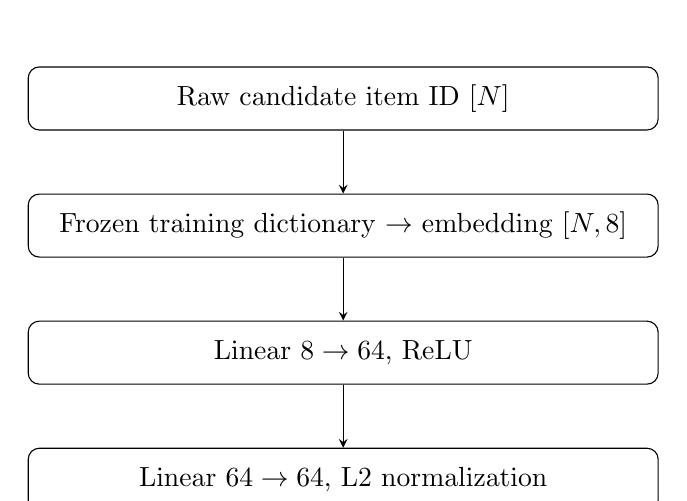
\begin{tikzpicture}[node distance=8mm,every node/.style={draw,rounded corners,align=center,minimum width=8cm,minimum height=8mm},>=stealth]
\node (a) {Raw candidate item ID $[N]$};
\node[below=of a] (b) {Frozen training dictionary $\rightarrow$ embedding $[N,8]$};
\node[below=of b] (c) {Linear $8\rightarrow64$, ReLU};
\node[below=of c] (d) {Linear $64\rightarrow64$, L2 normalization};
\draw[->](a)--(b);\draw[->](b)--(c);\draw[->](c)--(d);
\end{tikzpicture}\end{center}

\subsection{User tower}
\begin{center}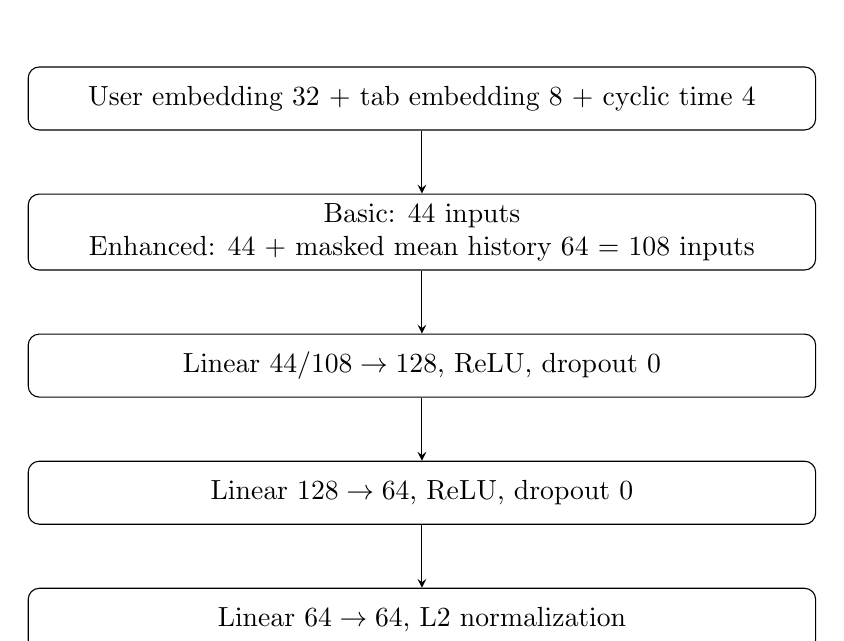
\begin{tikzpicture}[node distance=8mm,every node/.style={draw,rounded corners,align=center,minimum width=10cm,minimum height=8mm},>=stealth]
\node (a) {User embedding 32 + tab embedding 8 + cyclic time 4};
\node[below=of a] (b) {Basic: 44 inputs\\Enhanced: 44 + masked mean history 64 = 108 inputs};
\node[below=of b] (c) {Linear $44/108\rightarrow128$, ReLU, dropout 0};
\node[below=of c] (d) {Linear $128\rightarrow64$, ReLU, dropout 0};
\node[below=of d] (e) {Linear $64\rightarrow64$, L2 normalization};
\draw[->](a)--(b);\draw[->](b)--(c);\draw[->](c)--(d);\draw[->](d)--(e);
\end{tikzpicture}\end{center}

Batch normalization is disabled. History and targets share item-tower parameters, so gradients from the user-history pathway and positive targets both update the same item encoder. The basic path does not encode unused histories. A singleton final batch is consumed rather than dropped.

The historical item MLP has input width $8\times8+4=68$ and layers $68\rightarrow64\rightarrow64$. Its history-enhanced user width remains 108, but its item representations and source protocol differ.
\clearpage
\section{Loss, optimization and training budget}
For a batch of $B$ positive user-item pairs, let $D_i$ contain off-diagonal targets sharing the same item ID as target $i$. Training uses
\[\mathcal L=-{1\over B}\sum_{i=1}^B\log
{\exp(s(u_i,v_i)/\tau)\over\sum_{j\notin D_i}\exp(s(u_i,v_j)/\tau)},\qquad\tau=0.1.\]
The diagonal stays valid. Same-target off-diagonal entries are masked to $-\infty$ before cross-entropy. Different batch targets can still be false negatives: a user may also like them. No claim is made that these are observed dislikes. The initial baseline has no popularity/log-frequency correction for sampled comparisons.

\begin{table}[H]\centering
\begin{tabular}{ll}\toprule Configuration & Corrected basic and enhanced\\\midrule
Output dimension & 64, both towers normalized\\
Seed and shuffle & 42; deterministic global row permutation\\
Optimizer & Adam, $\beta_1=0.9$, $\beta_2=0.999$\\
Learning rate / weight decay & 0.001 / 0\\
Batch size / epochs & 256 / 1 full positive-sample traversal\\
Precision / device & CUDA AMP for the acceptance runs\\
Dropout / batch normalization & 0 / disabled\\
Temperature & 0.1\\
History (enhanced only) & At most 50 available positive items, masked mean\\
Logging / checkpoint & Every 50 / 500 steps, plus epoch-end checkpoint\\\bottomrule
\end{tabular}\caption{Frozen Week 1 training defaults. There is no validation-based hyperparameter search in this one-epoch comparison.}\end{table}

Checkpoint state includes model parameters, Adam state, AMP scaler, Python, NumPy, PyTorch and CUDA RNG states, epoch, next-batch cursor and consumed count. Publication writes the model before a checksummed completion marker. Recovery selects only intact completed checkpoint files and validates binding of code, configuration, data, runtime and device.

Validation in-batch loss depends on batch composition and the available denominator. It is not interchangeable with Recall@100 or NDCG@100, and a smaller last batch can have a mechanically smaller loss.
\clearpage
\section{Training results and provenance}
The completed Colab runs use Python 3.11.15, PyTorch 2.14.1+cu130 and an NVIDIA A100-SXM4-40GB. Both use seed 42, the same shuffled training positives and the frozen one-epoch configuration. Basic run ID is \texttt{5d0da236b294}; enhanced is \texttt{ce21055c8126}.
\begin{table}[H]\centering\small\begin{tabular}{lrrrrr}\toprule
Model & Consumed & Steps & Val. loss & Step+wait s & Peak MiB\\\midrule
basic & 124255 & 486 & 5.535129 & 7.243 & 83.85 \\
enhanced & 124255 & 486 & 5.530827 & 8.636 & 97.61 \\
\bottomrule\end{tabular}
\caption{Corrected-protocol training. Step+wait is the sum of logged batch data-wait and step durations, excluding checkpoint publication, validation and other orchestration. Peak memory is PyTorch allocated memory, not total GPU reservation or device usage.}\end{table}
\begin{figure}[H]\centering
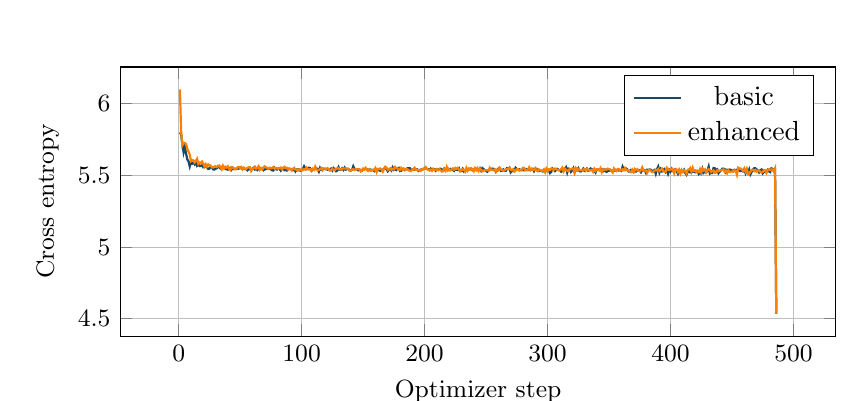
\begin{tikzpicture}\begin{axis}[width=.88\linewidth,height=5cm,xlabel={Optimizer step},ylabel={Cross entropy},grid=major,legend pos=north east,tick label style={font=\small},label style={font=\small}]
\addplot[color=accent,thick] coordinates {(1,5.80046082) (2,5.78750610) (3,5.71694946) (4,5.66194153) (5,5.69880676) (6,5.65315247) (7,5.61305237) (8,5.59860229) (9,5.56332397) (10,5.59495544) (11,5.58270264) (12,5.59053040) (13,5.57806396) (14,5.59590149) (15,5.56727600) (16,5.57608032) (17,5.56562805) (18,5.56504822) (19,5.57191467) (20,5.55737305) (21,5.56111145) (22,5.56466675) (23,5.55632019) (24,5.54525757) (25,5.54718018) (26,5.55895996) (27,5.55665588) (28,5.54188538) (29,5.54139709) (30,5.54644775) (31,5.54960632) (32,5.56320190) (33,5.55570984) (34,5.54843140) (35,5.56013489) (36,5.55766296) (37,5.54866028) (38,5.54461670) (39,5.54406738) (40,5.53991699) (41,5.55143738) (42,5.55282593) (43,5.53977966) (44,5.55357361) (45,5.54377747) (46,5.54676819) (47,5.54505920) (48,5.54551697) (49,5.54811096) (50,5.55436707) (51,5.54766846) (52,5.54600525) (53,5.54811096) (54,5.54382324) (55,5.54501343) (56,5.53599548) (57,5.54672241) (58,5.54222107) (59,5.54457092) (60,5.54748535) (61,5.55386353) (62,5.54087830) (63,5.54566956) (64,5.53749084) (65,5.54809570) (66,5.54641724) (67,5.54307556) (68,5.54660034) (69,5.53578186) (70,5.54217529) (71,5.54490662) (72,5.55007935) (73,5.54635620) (74,5.54719543) (75,5.54362488) (76,5.53536987) (77,5.53393555) (78,5.55226135) (79,5.54307556) (80,5.54075623) (81,5.54920959) (82,5.54489136) (83,5.53363037) (84,5.55126953) (85,5.54866028) (86,5.53678894) (87,5.54067993) (88,5.53405762) (89,5.54679871) (90,5.54373169) (91,5.54493713) (92,5.54217529) (93,5.53726196) (94,5.54817200) (95,5.52861023) (96,5.54151917) (97,5.54219055) (98,5.54232788) (99,5.53251648) (100,5.53753662) (101,5.54354858) (102,5.56323242) (103,5.54664612) (104,5.54280090) (105,5.54753113) (106,5.55345154) (107,5.55018616) (108,5.53233337) (109,5.54144287) (110,5.54461670) (111,5.55340576) (112,5.55039978) (113,5.54447937) (114,5.52671814) (115,5.55323792) (116,5.54048157) (117,5.54763794) (118,5.54397583) (119,5.54403687) (120,5.54307556) (121,5.54014587) (122,5.54077148) (123,5.53860474) (124,5.54739380) (125,5.53388977) (126,5.55029297) (127,5.53945923) (128,5.52893066) (129,5.53421021) (130,5.55735779) (131,5.53929138) (132,5.53936768) (133,5.54954529) (134,5.53846741) (135,5.55427551) (136,5.54006958) (137,5.54444885) (138,5.54563904) (139,5.53393555) (140,5.53515625) (141,5.53863525) (142,5.56323242) (143,5.54338074) (144,5.54426575) (145,5.54312134) (146,5.53533936) (147,5.54014587) (148,5.53562927) (149,5.53344727) (150,5.54382324) (151,5.54310608) (152,5.54562378) (153,5.54258728) (154,5.53532410) (155,5.54237366) (156,5.54089355) (157,5.53511047) (158,5.53903198) (159,5.53030396) (160,5.54275513) (161,5.54295349) (162,5.54414368) (163,5.53569031) (164,5.53190613) (165,5.53883362) (166,5.53823853) (167,5.54718018) (168,5.54733276) (169,5.54640198) (170,5.52911377) (171,5.53900146) (172,5.54595947) (173,5.53486633) (174,5.55538940) (175,5.53825378) (176,5.54272461) (177,5.53759766) (178,5.54608154) (179,5.55192566) (180,5.53033447) (181,5.53253174) (182,5.53959656) (183,5.54281616) (184,5.54045105) (185,5.54217529) (186,5.54983521) (187,5.55081177) (188,5.55058289) (189,5.53761292) (190,5.53848267) (191,5.54515076) (192,5.53889465) (193,5.54171753) (194,5.54238892) (195,5.53147888) (196,5.53744507) (197,5.54074097) (198,5.54096985) (199,5.54293823) (200,5.55075073) (201,5.54895020) (202,5.54405212) (203,5.54243469) (204,5.53689575) (205,5.54748535) (206,5.54035950) (207,5.54573059) (208,5.54371643) (209,5.53271484) (210,5.54429626) (211,5.54106140) (212,5.54380798) (213,5.54663086) (214,5.54042053) (215,5.53660583) (216,5.54849243) (217,5.54017639) (218,5.53984070) (219,5.54757690) (220,5.53791809) (221,5.54519653) (222,5.53868103) (223,5.53976440) (224,5.53201294) (225,5.54536438) (226,5.53926086) (227,5.53701782) (228,5.54856873) (229,5.52850342) (230,5.53071594) (231,5.54541016) (232,5.52774048) (233,5.53503418) (234,5.54058838) (235,5.53590393) (236,5.53938293) (237,5.54687500) (238,5.54782104) (239,5.53573608) (240,5.53823853) (241,5.55053711) (242,5.54518127) (243,5.53669739) (244,5.53703308) (245,5.54980469) (246,5.53305054) (247,5.55081177) (248,5.54368591) (249,5.53723145) (250,5.53128052) (251,5.52487183) (252,5.53315735) (253,5.54621887) (254,5.54234314) (255,5.54743958) (256,5.54598999) (257,5.54194641) (258,5.52447510) (259,5.53421021) (260,5.54826355) (261,5.55094910) (262,5.53178406) (263,5.53279114) (264,5.54142761) (265,5.53350830) (266,5.53146362) (267,5.54978943) (268,5.54489136) (269,5.55335999) (270,5.52169800) (271,5.53160095) (272,5.53053284) (273,5.52893066) (274,5.55279541) (275,5.54393005) (276,5.54299927) (277,5.54237366) (278,5.53808594) (279,5.53538513) (280,5.53977966) (281,5.53590393) (282,5.53825378) (283,5.54359436) (284,5.53688049) (285,5.54132080) (286,5.53614807) (287,5.54689026) (288,5.54643250) (289,5.52952576) (290,5.54632568) (291,5.54605103) (292,5.53211975) (293,5.53108215) (294,5.53150940) (295,5.53221130) (296,5.52752686) (297,5.52865601) (298,5.52983093) (299,5.53622437) (300,5.52908325) (301,5.53810120) (302,5.51658630) (303,5.52517700) (304,5.54785156) (305,5.54130554) (306,5.53030396) (307,5.53872681) (308,5.54489136) (309,5.53816223) (310,5.53671265) (311,5.52558899) (312,5.53092957) (313,5.53207397) (314,5.54394531) (315,5.55612183) (316,5.52035522) (317,5.54727173) (318,5.54421997) (319,5.52505493) (320,5.53546143) (321,5.55072021) (322,5.52105713) (323,5.54447937) (324,5.53643799) (325,5.54997253) (326,5.52981567) (327,5.52746582) (328,5.53610229) (329,5.54698181) (330,5.53216553) (331,5.53807068) (332,5.54708862) (333,5.53327942) (334,5.53695679) (335,5.54804993) (336,5.54367065) (337,5.53703308) (338,5.53341675) (339,5.52026367) (340,5.54235840) (341,5.54129028) (342,5.53569031) (343,5.53514099) (344,5.54321289) (345,5.52931213) (346,5.54080200) (347,5.52845764) (348,5.52471924) (349,5.53244019) (350,5.53152466) (351,5.53823853) (352,5.53439331) (353,5.52633667) (354,5.53359985) (355,5.53349304) (356,5.53308105) (357,5.54060364) (358,5.53422546) (359,5.53356934) (360,5.53100586) (361,5.56062317) (362,5.53964233) (363,5.53837585) (364,5.54747009) (365,5.53982544) (366,5.52787781) (367,5.53269958) (368,5.53811646) (369,5.53047180) (370,5.52377319) (371,5.54081726) (372,5.52778625) (373,5.53460693) (374,5.53446960) (375,5.53590393) (376,5.52203369) (377,5.53845215) (378,5.53868103) (379,5.53662109) (380,5.51847839) (381,5.53956604) (382,5.53715515) (383,5.54258728) (384,5.53961182) (385,5.53244019) (386,5.53048706) (387,5.53793335) (388,5.51144409) (389,5.54304504) (390,5.56056213) (391,5.52056885) (392,5.54338074) (393,5.52883911) (394,5.53816223) (395,5.54466248) (396,5.52360535) (397,5.53450012) (398,5.51103210) (399,5.53876495) (400,5.52671814) (401,5.54600525) (402,5.53280640) (403,5.54023743) (404,5.54362488) (405,5.52934265) (406,5.51132202) (407,5.53323364) (408,5.52015686) (409,5.53277588) (410,5.52908325) (411,5.53965759) (412,5.51719666) (413,5.50489044) (414,5.52307129) (415,5.53494263) (416,5.52116394) (417,5.52407837) (418,5.52359009) (419,5.52790833) (420,5.52214050) (421,5.53216553) (422,5.53053284) (423,5.50978088) (424,5.51832581) (425,5.51162720) (426,5.54519653) (427,5.51953125) (428,5.52781677) (429,5.52075958) (430,5.53315735) (431,5.56138611) (432,5.51246643) (433,5.51847839) (434,5.51693726) (435,5.55139923) (436,5.54965210) (437,5.53907776) (438,5.54295349) (439,5.51518250) (440,5.52574921) (441,5.53478241) (442,5.54621887) (443,5.54734802) (444,5.54408264) (445,5.52362823) (446,5.53869629) (447,5.53466797) (448,5.54045105) (449,5.53927612) (450,5.53408813) (451,5.52797699) (452,5.53886414) (453,5.53476715) (454,5.53974915) (455,5.54008484) (456,5.53282166) (457,5.53100586) (458,5.53425598) (459,5.52833557) (460,5.54411316) (461,5.51613617) (462,5.53738403) (463,5.51773071) (464,5.54090881) (465,5.50772095) (466,5.52496338) (467,5.54148865) (468,5.54981995) (469,5.55026245) (470,5.54154968) (471,5.53514099) (472,5.52088928) (473,5.53492737) (474,5.54116821) (475,5.51444244) (476,5.52407837) (477,5.53196716) (478,5.52580261) (479,5.53837585) (480,5.52847290) (481,5.52352905) (482,5.54890442) (483,5.54592896) (484,5.53147888) (485,5.53729248) (486,4.53509474)};\addlegendentry{basic}
\addplot[color=orange,thick] coordinates {(1,6.10007477) (2,5.80721283) (3,5.71003723) (4,5.72691345) (5,5.72564697) (6,5.71856689) (7,5.68690491) (8,5.66560364) (9,5.64567566) (10,5.59913635) (11,5.60702515) (12,5.60417175) (13,5.59107971) (14,5.59931946) (15,5.61474609) (16,5.58038330) (17,5.58979797) (18,5.58569336) (19,5.59664917) (20,5.58216858) (21,5.56195068) (22,5.57789612) (23,5.56108093) (24,5.57687378) (25,5.57048035) (26,5.56854248) (27,5.55732727) (28,5.55525208) (29,5.56088257) (30,5.56465149) (31,5.55886841) (32,5.56402588) (33,5.56958008) (34,5.55776978) (35,5.54246521) (36,5.56683350) (37,5.54861450) (38,5.56077576) (39,5.55480957) (40,5.56283569) (41,5.54537964) (42,5.53785706) (43,5.55789185) (44,5.55401611) (45,5.54696655) (46,5.54219055) (47,5.54434204) (48,5.55799866) (49,5.55918884) (50,5.55235291) (51,5.55871582) (52,5.54162598) (53,5.55416870) (54,5.54652405) (55,5.54621887) (56,5.55378723) (57,5.55746460) (58,5.55657959) (59,5.53120422) (60,5.54522705) (61,5.55137634) (62,5.56079102) (63,5.54646301) (64,5.55221558) (65,5.56413269) (66,5.53933716) (67,5.55157471) (68,5.54200745) (69,5.55551147) (70,5.56346130) (71,5.55633545) (72,5.55216980) (73,5.54577637) (74,5.55354309) (75,5.54975891) (76,5.55099487) (77,5.55818176) (78,5.54731750) (79,5.55101013) (80,5.54872131) (81,5.54696655) (82,5.55152893) (83,5.55496216) (84,5.54122925) (85,5.55117798) (86,5.55928040) (87,5.55114746) (88,5.55326843) (89,5.54110718) (90,5.54844666) (91,5.54429626) (92,5.53422546) (93,5.54743958) (94,5.54939270) (95,5.54081726) (96,5.53851318) (97,5.53334045) (98,5.54234314) (99,5.53689575) (100,5.54440308) (101,5.53645325) (102,5.54354858) (103,5.54011536) (104,5.55461121) (105,5.54370117) (106,5.54025269) (107,5.54292297) (108,5.53376770) (109,5.54608154) (110,5.53933716) (111,5.56117249) (112,5.54116821) (113,5.53643799) (114,5.53701782) (115,5.54406738) (116,5.55058289) (117,5.53628540) (118,5.54896545) (119,5.54890442) (120,5.54547119) (121,5.55125427) (122,5.54597473) (123,5.53330994) (124,5.53713989) (125,5.54534912) (126,5.53849792) (127,5.53698730) (128,5.54762268) (129,5.54728699) (130,5.55094910) (131,5.54165649) (132,5.54039001) (133,5.54586792) (134,5.54888916) (135,5.54849243) (136,5.54826355) (137,5.54847717) (138,5.54362488) (139,5.53456116) (140,5.53091431) (141,5.54060364) (142,5.54382324) (143,5.53779602) (144,5.54293823) (145,5.54458618) (146,5.54391479) (147,5.54307556) (148,5.52833557) (149,5.53628540) (150,5.54776001) (151,5.54043579) (152,5.55313110) (153,5.54011536) (154,5.53182983) (155,5.54290771) (156,5.53251648) (157,5.53804016) (158,5.53878784) (159,5.53724670) (160,5.55117798) (161,5.52432251) (162,5.54452515) (163,5.54579163) (164,5.54855347) (165,5.54168701) (166,5.52618408) (167,5.54646301) (168,5.56060791) (169,5.55451965) (170,5.53889465) (171,5.54508972) (172,5.54756165) (173,5.53976440) (174,5.54560852) (175,5.54180908) (176,5.55879211) (177,5.55003357) (178,5.54910278) (179,5.54202271) (180,5.53726196) (181,5.55241394) (182,5.54119873) (183,5.54809570) (184,5.53591919) (185,5.54435730) (186,5.54493713) (187,5.53466797) (188,5.53054810) (189,5.53105164) (190,5.54141235) (191,5.53866577) (192,5.55239868) (193,5.53886414) (194,5.53996277) (195,5.53550720) (196,5.53764343) (197,5.53178406) (198,5.54447937) (199,5.54324341) (200,5.54443359) (201,5.55755615) (202,5.54594421) (203,5.53900146) (204,5.53529358) (205,5.54089355) (206,5.53155518) (207,5.54560852) (208,5.53964233) (209,5.53762817) (210,5.54344177) (211,5.53651428) (212,5.54473877) (213,5.53701782) (214,5.52664185) (215,5.52861023) (216,5.54502869) (217,5.53228760) (218,5.55953979) (219,5.53469849) (220,5.54257202) (221,5.53488159) (222,5.54067993) (223,5.54988098) (224,5.54052734) (225,5.55215454) (226,5.54574585) (227,5.55284119) (228,5.53982544) (229,5.53054810) (230,5.53596497) (231,5.54286194) (232,5.53819275) (233,5.52635193) (234,5.55290222) (235,5.53321838) (236,5.54785156) (237,5.54054260) (238,5.54849243) (239,5.54066467) (240,5.52909851) (241,5.55024719) (242,5.53654480) (243,5.54975891) (244,5.53088379) (245,5.54724121) (246,5.53811646) (247,5.52905273) (248,5.53347778) (249,5.53622437) (250,5.53585815) (251,5.53633118) (252,5.53413391) (253,5.55303955) (254,5.53784180) (255,5.53956604) (256,5.53640747) (257,5.54179382) (258,5.52627563) (259,5.54013062) (260,5.53553772) (261,5.55392456) (262,5.54225159) (263,5.53569031) (264,5.53306580) (265,5.53697205) (266,5.54296875) (267,5.54301453) (268,5.54463196) (269,5.55239868) (270,5.54127502) (271,5.53631592) (272,5.54331970) (273,5.52879333) (274,5.53517151) (275,5.54391479) (276,5.54408264) (277,5.53347778) (278,5.53730774) (279,5.53820801) (280,5.55316162) (281,5.55261230) (282,5.53495789) (283,5.53771973) (284,5.53979492) (285,5.55651855) (286,5.53796387) (287,5.54522705) (288,5.54164124) (289,5.53797913) (290,5.54988098) (291,5.53399658) (292,5.52912903) (293,5.54133606) (294,5.53610229) (295,5.53163147) (296,5.53363037) (297,5.54278564) (298,5.52233887) (299,5.54788208) (300,5.53120422) (301,5.54171753) (302,5.53839111) (303,5.54820251) (304,5.54347229) (305,5.53686523) (306,5.54804993) (307,5.54591370) (308,5.53750610) (309,5.53562927) (310,5.53585815) (311,5.54403687) (312,5.55456543) (313,5.52803040) (314,5.54704285) (315,5.53994751) (316,5.53283691) (317,5.52967834) (318,5.54513550) (319,5.54266357) (320,5.54797363) (321,5.54849243) (322,5.52003479) (323,5.55027771) (324,5.53720093) (325,5.54530334) (326,5.53773499) (327,5.53576660) (328,5.53500366) (329,5.54135132) (330,5.54454041) (331,5.53234863) (332,5.54360962) (333,5.53800964) (334,5.53401184) (335,5.53637695) (336,5.53947449) (337,5.52529907) (338,5.54597473) (339,5.53105164) (340,5.54243469) (341,5.54269409) (342,5.53562927) (343,5.55056763) (344,5.52339172) (345,5.53985596) (346,5.53738403) (347,5.54289246) (348,5.54058838) (349,5.54736328) (350,5.54420471) (351,5.54035950) (352,5.53285217) (353,5.52061462) (354,5.54875183) (355,5.54005432) (356,5.53106689) (357,5.54423523) (358,5.54519653) (359,5.53355408) (360,5.53663635) (361,5.54286194) (362,5.53620911) (363,5.55198669) (364,5.53649902) (365,5.53839111) (366,5.53489685) (367,5.52320862) (368,5.52210999) (369,5.53916931) (370,5.52397156) (371,5.54457092) (372,5.53623962) (373,5.54289246) (374,5.53292847) (375,5.52894592) (376,5.53785706) (377,5.55566406) (378,5.53254700) (379,5.53349304) (380,5.53471375) (381,5.51788330) (382,5.53472900) (383,5.54067993) (384,5.53153992) (385,5.52291870) (386,5.52484131) (387,5.53385925) (388,5.53663635) (389,5.53514099) (390,5.54498291) (391,5.53085327) (392,5.53634644) (393,5.54776001) (394,5.53231812) (395,5.52560425) (396,5.52536011) (397,5.55235291) (398,5.54046631) (399,5.53741455) (400,5.54258728) (401,5.54672241) (402,5.53433228) (403,5.51374817) (404,5.54454041) (405,5.54129028) (406,5.52343750) (407,5.53962708) (408,5.51335144) (409,5.53764343) (410,5.52413940) (411,5.53746033) (412,5.52952576) (413,5.51284790) (414,5.53819275) (415,5.54145813) (416,5.55065918) (417,5.52536011) (418,5.55343628) (419,5.53140259) (420,5.53517151) (421,5.52412415) (422,5.53117371) (423,5.52420044) (424,5.54423523) (425,5.52023315) (426,5.54675293) (427,5.53472900) (428,5.54205322) (429,5.52052307) (430,5.53659058) (431,5.54411316) (432,5.53694153) (433,5.52326965) (434,5.52961731) (435,5.53433228) (436,5.51843262) (437,5.52082825) (438,5.53602600) (439,5.52812195) (440,5.53289795) (441,5.53639221) (442,5.53877258) (443,5.54168701) (444,5.52384949) (445,5.53279114) (446,5.51631165) (447,5.53587341) (448,5.52400208) (449,5.52615356) (450,5.52726746) (451,5.52575684) (452,5.53631592) (453,5.53038025) (454,5.50497437) (455,5.55397034) (456,5.54924011) (457,5.54878235) (458,5.54121399) (459,5.53048706) (460,5.54779053) (461,5.52638245) (462,5.54588318) (463,5.51130676) (464,5.51249695) (465,5.52616882) (466,5.53843689) (467,5.54002380) (468,5.52967834) (469,5.53802490) (470,5.52673340) (471,5.53486633) (472,5.53558350) (473,5.52445984) (474,5.52058411) (475,5.52415466) (476,5.53704834) (477,5.53164673) (478,5.51699829) (479,5.53669739) (480,5.54354858) (481,5.53751373) (482,5.54209900) (483,5.54084778) (484,5.52796936) (485,5.54850769) (486,4.53840446)};\addlegendentry{enhanced}
\end{axis}\end{tikzpicture}\caption{Actual corrected-protocol training losses. Step 486 contains only 95 examples; its lower loss must not be interpreted as sudden learning progress.}\end{figure}
The first 485 batches contain 256 examples each, while the final batch contains 95. Uniform logits would have cross entropy approximately $\ln256=5.545$ versus $\ln95=4.554$, before duplicate-target masking. Actual final losses are 4.535095 (basic) and 4.538404 (enhanced). The mean loss of the last 20 full batches is 5.534524 and 5.533771 respectively. Recomputed uniform-logit validation loss with the same shuffled batches and duplicate mask is approximately 5.540678; the observed validation losses are only slightly lower. Loss measures discrimination within sampled batches, not full-catalog recommendation quality.

Both exports contain all 7,583 catalog IDs and 64-dimensional, finite unit-norm vectors. Export bindings match the corresponding checkpoints and frozen data/code/configuration identities. The private Drive retains complete checkpoints, vectors and request-level predictions; W\&B retains training logs. The recovery run \texttt{723f7c5b353e} is an acceptance experiment, not a third predictive model, despite sharing the enhanced display name.

The original run \texttt{b2ed5728b9a2} consumed 124,780 positives in 488 steps with validation in-batch loss 5.516606. These historical measurements use the original duplicate/history/content rules and remain outside the fair comparison.
\clearpage
\section{Evaluation protocol and measured results}
Validation requests are all retained nonrandom positive exposures in the frozen validation window. The same request identities, catalog and eligibility rule apply to all three corrected-protocol systems. Available earlier validation feedback may enter later histories without updating model parameters. Repeat-view candidates are allowed.

Upload dates have day precision. An item becomes eligible at 00:00 UTC on the day after its upload date. Missing eligibility dates are excluded and counted. This is a conservative publication-date proxy; historical removals and visibility changes cannot be reconstructed from the snapshot.

\begin{table}[H]\centering\small\begin{tabular}{lrrrrr}\toprule
Model & Requests & Recall@100 & NDCG@100 & Coverage & Short lists\\\midrule
popularity & 30589 & 0.270784 & 0.069607 & 100.00\% & 0.00\% \\
basic & 30589 & 0.020301 & 0.005489 & 100.00\% & 0.00\% \\
enhanced & 30589 & 0.019288 & 0.004112 & 100.00\% & 0.00\% \\\bottomrule\end{tabular}
\caption{Corrected-protocol exact retrieval. Unavailable targets are retained in the metric denominator.}\end{table}

\subsection{Explicit numerator, denominator and ranking standard}
Standard/nonrandom means \texttt{is\_random=0}: exposure selected by the original recommendation policy rather than the dataset's randomized exposure mechanism. Each retained validation record with \texttt{long\_view=1} is one request, with its user, request time and one observed positive target. The target is withheld from the recommendation scoring inputs; user history contains only feedback available before that request.

For popularity, item score is the number of nonrandom long-view records for that item in the training window. Validation labels never contribute to these counts. For either tower model, score is normalized user--item dot product. All systems use identical request identities and eligible candidates, score descending with raw item ID ascending for ties. In this dataset all 7,583 candidates are already time-eligible throughout validation; popularity consequently produces the same list for every request, while neural lists depend on user context.

\textbf{Numerator:} the number of validation requests whose actual target occurs in that request's predicted Top-100. \textbf{Denominator:} all 30,589 retained validation-positive requests, including any uncovered targets. The number 100 is the recommendation-list cutoff, not the denominator. A request with its target at rank 1, 10 or 100 counts as one hit; rank 101 counts as zero. NDCG additionally rewards earlier ranks: contributions are 1, approximately 0.289 and 0.150 at those three hit positions.

\begin{table}[H]\centering\small\begin{tabular}{lrrr}\toprule
Model & Hit requests & All requests & Recall@100 (\%)\\\midrule
Popularity & 8283 & 30589 & 27.0784\\
Basic & 621 & 30589 & 2.0301\\
Enhanced & 590 & 30589 & 1.9288\\\bottomrule\end{tabular}
\caption{Integer numerators independently recomputed from private request-level predictions.}\end{table}
This is a request-weighted aggregate, not a mean of per-user recalls: a user with more positive requests contributes more observations. Repeated users and repeated target videos are not deduplicated across requests. Per-user averages and user-level distributions have not yet been measured. Recommended non-target items are not confirmed dislikes; this single-target protocol cannot assess all potentially relevant videos.

For one relevant target per request, with rank $r_q$,
\[\operatorname{Recall@100}=\operatorname{HitRate@100}={1\over Q}\sum_q\mathbf1[r_q\le100],\]
\[\operatorname{NDCG@100}={1\over Q}\sum_q{\mathbf1[r_q\le100]\over\log_2(r_q+1)}.\]
A target absent from the eligible candidate set is a miss. Covered-only metrics are secondary diagnostics, not replacements for the end-to-end result. Empty slices use null rather than a fabricated zero.

Scores are computed by bounded request/item matrix blocks. Each block is merged into an exact Top-100 using score-descending, raw-ID-ascending sorting, including boundary ties. Missing result slots are explicit $-1$ sentinels. Vector shards must cover the full manifest catalog exactly, without duplicate IDs, and match the checkpoint's binding and unit norm requirement.
\subsection{Observed comparison and its interpretation}
Popularity is substantially stronger than both towers. Enhanced hits 590 requests versus 621 for basic: 31 fewer hits, approximately 5.0\% lower Recall and 25.1\% lower NDCG. The observed mean-history enhancement does not demonstrate a benefit in this run. No significance or stability claim is made from one seed. As a mathematical reference only, uniform sampling of 100 distinct candidates from 7,583 would have expected single-target hit probability $100/7583\approx1.319\%$; no random recommender was executed.

The weak tower results are consistent with their near-uniform in-batch validation loss, but they do not identify a unique root cause. One epoch, sparse per-user training positives, an 8-dimensional item-ID embedding, mean history pooling and uncorrected in-batch sampling merit separate diagnostics. These are hypotheses, not established implementation bugs. Standard-policy exposure can favor popular items in both periods; offline success is not an unbiased estimate of online improvement. Training labels are legitimate learning inputs, whereas using validation labels to construct the popularity scores would be leakage.
\clearpage
\section{Coverage, performance and reliability}
The corrected validation package contains 3.97\% unknown-user requests and 1.49\% empty-history requests. The measured candidate target coverage is 100.00\%; no positive target is silently dropped for unsupported users or missing eligibility.

All current timings below come from the completed Colab evaluation, with request batches of 256 and one excluded warmup batch. User encoding uses CUDA for the towers; exact matrix scoring and sorting run on CPU for every model. A \texttt{device=cuda} field therefore does not mean GPU retrieval.
\begin{table}[H]\centering\small\begin{tabular}{lrrrr}\toprule
Model & Encode s & Retrieve s & Batch P50 s & Batch P95 s\\\midrule
popularity & 0.002474 & 13.566819 & 0.113596 & 0.116308 \\
basic & 0.426576 & 25.620920 & 0.207204 & 0.277423 \\
enhanced & 0.565114 & 25.485775 & 0.208044 & 0.269540 \\
\bottomrule\end{tabular}\caption{Measured Colab batch timings; neither production single-request latency nor a GPU retrieval benchmark.}\end{table}
Timing includes user feature assembly, user encoding, GPU-to-CPU transfer where applicable and CPU exact retrieval, excluding initial model/data loading. Popularity's simpler count scoring requires less work than 64-dimensional neural dot products. The prior local CPU popularity timing of 8.103 seconds belongs to a different hardware execution and is not substituted for the Colab measurements.

Covered-only Recall and NDCG equal their end-to-end values for all three models because target coverage is 100\%. Short-list rate is zero. Unknown-user requests number 1,213 (3.9655\%); empty-history requests number 456 (1.4907\%). These describe the shared evaluation requests, not model-specific failures. Catalog unknown item-category rate (9.2444\%) and validation-target unknown category rate (0.1112\%) use different denominators and are distinct from catalog target coverage.

\subsection{Historical checkpoint diagnostic}
Frozen-source CPU diagnostic inference on the original 30,780 validation positives yields Recall@100 0.023717 and NDCG@100 0.006615. This is not part of the corrected comparison: the old model was trained with original duplicates, request-prior histories and snapshot content. It cannot certify the new protocol or be used to infer a fair improvement over the new popularity baseline.

\subsection{Correctness and acceptance}
Tests cover hand-calculated rank metrics, block/full equivalence, deterministic ties, temporal eligibility, uncovered targets, short lists, duplicate candidate IDs, completion-time histories, same-millisecond requests, unknown users and empty history. Model integration tests verify ID-only feature exclusion, normalized vectors, strict checkpoint binding and deterministic CPU recovery.

The controlled CUDA recovery check passed: training stopped after step 25, saved next-batch cursor 25, restored the checkpoint and completed 486 steps with 124,255 consumed samples. Final model, Adam, AMP scaler, Python/NumPy/PyTorch/CUDA RNG states and cursors match the uninterrupted enhanced reference exactly ($\mathrm{rtol}=0$, $\mathrm{atol}=0$). Final checkpoint file hashes differ because serialization and run metadata differ; state equality, rather than byte equality, is the acceptance condition. This test runs within the same runtime and does not demonstrate recovery after Colab disconnection or a newly provisioned runtime.

Independent post-run checks matched all request IDs and targets against frozen validation, recomputed hit counts and NDCG from predictions, verified 100 unique eligible recommendations per request, reconstructed popularity ranking from training counts and checked prediction/evaluation/release hashes. These checks did not independently replay neural scoring from checkpoint tensors.

\subsection{Stage status and remaining evidence}
The release reports \texttt{complete=true} and no artifact blockers. Both full CUDA baseline runs, matching exports, all three evaluations and controlled recovery evidence are present. Remaining evidence includes recovery in a fresh Colab runtime, user-level/sliced metrics, multiple-seed stability and online or random-exposure validation. The sealed test remains unused. Poor neural performance is an experiment outcome, not a failure of the artifact completion gate.
\clearpage
\section{Week 2 work and experiment discipline}
\begin{table}[H]\centering\small
\begin{tabularx}{\linewidth}{lXX}\toprule
Workstream & Next task & Acceptance evidence\\\midrule
Data & Publish audited 27K data and stable nested user subsets; investigate date semantics and metadata provenance & Source/row reconciliation, fixed subset hashes, no future history\\
User model & Compare no-history versus masked mean history with the shared trainer & Same budget, seed, requests and candidate protocol\\
Item model & Admit content only with defensible as-of provenance; compare ID-only versus content & Frozen train-only transformations and explicit feature availability\\
Joint experiments & Run basic, history-only, item-content-only and combined configurations & Four comparable validation results and cost measurements\\
Evaluation & Add long-tail, cold-start and eligibility coverage slices & Frozen definitions, per-slice counts, null for empty groups\\
Scaling & Estimate full traversal and encoding cost from measured throughput & Explicit GPU type, memory and data-wait measurements\\\bottomrule
\end{tabularx}\caption{Week 2 priorities. ANN work follows a validated exact-retrieval reference.}\end{table}

Do not widen the search to multiple model depths, dimensions and losses simultaneously. Keep the full traversal budget fixed for the four principal comparisons. Use validation Recall@100 for later selection, retain NDCG@100 and coverage, and preserve all runs including non-improvements.

The final test bundle remains unused for training, tuning and stage selection. Candidate/request changes are versioned; results across changed protocols are not described as direct model improvements. Learned scores remain retrieval scores until a separate calibration or ranking task is established.

\subsection{Known limitations}
\begin{enumerate}
\item Recorded date disagrees with fixed UTC and UTC+08 calendars; date is not used for splitting.
\item No logged feedback-completion timestamp; full observed playback used as conservative proxy.
\item Metadata is an unversioned snapshot; content features excluded, upload date used only as a catalog eligibility proxy.
\item Pure histories omit videos outside the candidate pool; standard-exposure validation is not an unbiased online estimate.
\item One seed and one epoch provide a baseline, not a stability estimate or evidence of optimal convergence.
\item The item ID embedding cannot supply content generalization for unseen training items; the reserved unknown category is not a trained content representation.
\item Batch comparisons can contain false negatives, and the initial loss has no popularity correction.
\end{enumerate}
\clearpage
\textbf{Executed source commit:} \path{c29eb4571556ef7e27a636f3af48e6ce7d1775c4}

\appendix\section{Feature examples and reproduction contract}
\begin{table}[H]\centering\small\begin{tabularx}{\linewidth}{lXrrr}\toprule
Field & Actual values & Values & Min & Max\\\midrule
\texttt{user\_user\_id} & 20853 & 26938 & 0 & 27,284 \\
\texttt{user\_tab} & 1 & 15 & 0 & 14 \\
\texttt{user\_time\_ms} & 1649475963278 & 1269263 & 1,649,475,963,278 & 1,651,622,398,321 \\
\texttt{long\_view} & 0 & 2 & 0 & 1 \\
\texttt{play\_time\_ms} & 1286 & 151346 & 0 & 964,774 \\
\texttt{duration\_ms} & 289866 & 5737 & 0 & 1,177,720 \\\bottomrule\end{tabularx}\caption{Actual retained warmup/train/validation event examples; anonymous public IDs are not personal identities. User-prefixed names disambiguate event fields from item metadata.}\end{table}

Training batches contain $[B]$ tensors for user ID, target item ID, time, scenario and official label; history item IDs and mask are $[B,50]$. The formal ID-only item tower ignores standardized compatibility columns \texttt{category} and \texttt{duration}. Nonrandom positive filtering uses \texttt{long\_view} and \texttt{is\_random}; request ID and split are protocol fields rather than learned features.

\begin{description}
\item[Prepared manifest SHA-256] \hfill\\\path{0c35d9c9f483bca90f909cd8bcf5f7f1c6c64e6c3aeea411ea3617d0cc92b7fc}
\item[Validation request identity hash] \hfill\\\path{c622789c33544e0122abb8d151ff22a50d8bd2db91a99589fddfba6e7db28efd}
\item[Candidate artifact hash] \hfill\\\path{9b49e12466f88e9cbf0634b0f8e767104d17a7a4145b7bd730d2275d638c636d}
\item[Official raw archive SHA-256] \hfill\\\path{c814bf6f3624c0cfae83c57de3df26b2ed206e5c57bab4c4dcbfabbabe20cbf0}
\end{description}

The team Drive separates raw data, versioned datasets, experiment runs and frozen releases by project and stage. The public notebook is \texttt{week1\_baseline.ipynb}. It reads mounted prepared files directly. Optional copying to \texttt{/content} is a performance cache and does not re-download the source dataset.

Rebuild this report with \texttt{build\_report.py}, providing the audit, matching manifest, stage release and real run-log root. Final generation refuses incomplete stages. Compilation uses an isolated temporary directory; auxiliary files are removed automatically. The standalone source includes its plot data and architecture diagrams.

\begin{thebibliography}{9}
\bibitem{kuairand} C. Gao et al. \emph{KuaiRand: An Unbiased Sequential Recommendation Dataset with Randomly Exposed Videos}. CIKM 2022, pp. 3953--3957. \url{https://arxiv.org/abs/2208.08696}.
\bibitem{dataset} KuaiRand project. Official dataset definitions and downloads. \url{https://kuairand.com/}.
\end{thebibliography}

\clearpage\section{Actual historical feature transformations}

For historical candidate ID 0, these values reproduce the frozen encoder. Numeric values are checked against the stored training median, mean and standard deviation; no held-out fitting is performed.

\begin{center}\small\begin{tabularx}{\linewidth}{lrrX}\toprule Feature & Raw value & Encoded value & Representation\\\midrule
item\_id & 0 & 1 & categorical dictionary index \\
author\_id & 7349781 & 4199 & categorical dictionary index \\
video\_type & NORMAL & 2 & categorical dictionary index \\
upload\_type & LongImport & 5 & categorical dictionary index \\
visible\_status & 0.0 & 1 & categorical dictionary index \\
music\_id & 9155697141 & 4461 & categorical dictionary index \\
music\_type & 9.0 & 5 & categorical dictionary index \\
tag & 39 & 61 & categorical dictionary index \\
video\_duration & 87433.0 & -0.193732 & training-imputed z-score \\
server\_width & 720.0 & -0.557563 & training-imputed z-score \\
server\_height & 1280.0 & 0.561088 & training-imputed z-score \\
upload\_day & 1 & 0.284630 & training-imputed z-score \\\bottomrule\end{tabularx}\end{center}

Under the corrected ID-only dictionary, 9.24\% of catalog items and 0.11\% of validation targets map to the reserved unknown item category. These differ from targets outside the eligible catalog. All valid candidate IDs remain in retrieval.

\section{Completed evaluation release identities}
The completed release is \texttt{week1-pure-completion-v1-001}, executed on 12 October 2026. Source and data identities below bind the comparison; historical artifacts remain separate.
\begin{description}
\item[Stage report SHA-256] \hfill\\\path{4c14b0ac9bf87f6abc60c1080b8b94d5d82184a6784b3ad88e5df006bfbdc469}
\item[Training code SHA-256] \hfill\\\path{143327677ec3df4098cb40a4210f8991398c3b41e25e29c646babe63f4bf47ff}
\item[Evaluator SHA-256] \hfill\\\path{a031fca9db8ae4099d93331162074c9522554b72947e43f77d185703c1f64ee9}
\item[basic configuration SHA-256] \hfill\\\path{0c2a71e707379e357b4df72778f6dce04b3f6640fa7174a7e9d5639250445cf7}
\item[basic checkpoint SHA-256] \hfill\\\path{acbeb4c9153a6a5901fa79be08d6d7f16f5520736e75fa0a32b21b633be34272}
\item[basic vector manifest SHA-256] \hfill\\\path{4b9248885cc9d022a2dd46e2665a272884b39b8cf3c302fde0c178fb8130d3f1}
\item[enhanced configuration SHA-256] \hfill\\\path{94d4c29a3727938f3fa8ee58732ef3bfeab36937437932e74df347ed0867730c}
\item[enhanced checkpoint SHA-256] \hfill\\\path{92d34958b807e3a5b8fefda8bf5a9d476b41cef589d88d76995c1e5a90024490}
\item[enhanced vector manifest SHA-256] \hfill\\\path{95823d65151a7cf206d71a4a8cda742a188319d5033bb20feefb32f8b2526e6e}
\item[popularity predictions SHA-256] \hfill\\\path{6a133a5a90285fb6a0ac2bb3326eb893d23363e5b58eb84646fd343d9b6de029}
\item[basic predictions SHA-256] \hfill\\\path{96e4d549ec35c67647d2f79f07f471f125327011c895936467b419ca9d3d2de3}
\item[enhanced predictions SHA-256] \hfill\\\path{1e8c44f8a961ed307f54432a89cf05f15488186592e1a21b9eaa5d741e7dd1a7}
\item[Recovered checkpoint SHA-256] \hfill\\\path{f893155ffddaadad414afd5662ccfb58ff264f5c08bc07a06ea127aa78e19cd8}
\end{description}
Notebook: \url{https://colab.research.google.com/drive/1rQwo_Fe_HufE3q7VvA1RTNmPiDBHQ_Yv}.\\
Release: \url{https://drive.google.com/drive/folders/1e19AK-3KjZf6Oi4IVj_g-4N6OzbUnGzQ}.\\
Basic log: \url{https://wandb.ai/SAR-Lab/kuairand-two-tower/runs/5d0da236b294}.\\
Enhanced log: \url{https://wandb.ai/SAR-Lab/kuairand-two-tower/runs/ce21055c8126}.\\
Recovery log: \url{https://wandb.ai/SAR-Lab/kuairand-two-tower/runs/723f7c5b353e}.

\end{document}
